\documentclass{article}
\usepackage[utf8]{inputenc}
\usepackage[margin=2.5cm]{geometry}
\usepackage[version=4]{mhchem}
\usepackage{graphicx}
\usepackage{hyperref}
\usepackage{wrapfig}
\usepackage{placeins}
\usepackage{subcaption}

\setlength\parindent{0pt}

\begin{document}

\begin{titlepage}
    \begin{center}
        \vspace*{1cm}
        \Huge
        \textbf{Transformation of potassium benzoate into benzoic acid}
        
        \vspace{0.5cm}
        \LARGE
        Chemistry 2 - TP 4
        
        \vspace{1.5cm}
        \textbf{Louis-Hendrik Barboutie}
        
        \text{StudID: 020157041C}
        
        \vfill
        
        
\includegraphics[width=0.4\textwidth]{logo_uni.jpg}
        
        \Large
        27$^{\underline{\text{th}}}$ April and 4$^{\underline{\text{th}}}$ May 2022
    \end{center}
\end{titlepage}

\section{Abstract}

The aim of this lab class was the liquid-liquid extraction of benzoic acid from a potassium benzoate solution and the study of the extracted substance via melting point analysis and infrared spectroscopy. The extraction was successful, resulting in a pure product with 54.78 \% yield.

\section{Introduction}

The goal of this experiment is, in a first step, to familiarize with the procedure of liquid-liquid extraction, and with the transformation of potasssium benzoate into benzoic acid. In a second step the the goal is to identify the obtained products via study of the melting point and IR spectrum.

The potassium benzoate is first dissolved in water. Adding hydrochloric acid, the products react and form potassium chloride and benzoic acid, as seen in eq.~\ref{eq:benzoicAcidReact} \cite{labguide} \cite{potassiumBenzoate} 

\begin{equation}
    \ce{C7H5KO2 + HCl -> C7H6O2 + KCl}
    \label{eq:benzoicAcidReact}
\end{equation}

By adding another solvent, diethyl ether, to the solution, two phases are created: the two liquids don't mix and are clearly distinguishable. The diethyl ether floats on top of the water. This is essential for the liquid-liquid extraction, since it consists of extracting the product from one liquid to another, therefore both liquids should not mix. Benzoic acid dissolves better in diethyl ether, so it will naturally transfer to the the diethyl ether phase \footnote{Benzoic acid has very low solubility in water, while it has very good solubility in ethanol and acetone \cite{benzoicAcid}}, while the other reactants and products stay in the aqueous phase. This enables us to only recover benzoic acid, by draining the aqueous phase. 

The advantage of using diethyl ether as secondary solvent is that it is less dense than water \cite{diethylEther}\cite{water}, and therefore lies on top of the aqueous phase during the experiment. If dichloromethane were to be used, it would lie beneath the aqueous phase, since it is more dense than water \cite{dichloromethane}.

The nature of the extracted product can then be verified by a multitude of ways, but two simple ones are the identification of the melting point and the study of the IR spectrum. The melting point varies for different substances, and can be a good ballpark indicator if the extracted product is the one desired. This is easily applicable only to substances that are solid at room temperature and have melting points in the range of 100-400°C. For more precise identification of the substances in a product, the IR spectroscopy is necessary, as each substance has a unique spectrum. This allows us to verify the purity of the product, and identify additional unwanted substances.

\section{Experiment}

\subsection{Setup and procedure}

For the liquid-liquid extraction, the potassium benzoate is first dissolved in water and then hydrochloric acid is added. The obtained product doesn't fully dissolve, but forms a white, cloudy liquid. It is then introduced in the separatory funnel seen in fig~\ref{fig:sepFunnel}, and diethyl ether is added, to begin the extraction. The container with potassium benzoate is rinsed with water several times and added to the funnel, in order to get the most amount possible of potassium benzoate into the funnel. When extracting, to make sure most of the benzoic acid gets into the diethyl ether phase, the separatory funnel is shaken several times under a fumehood.

The separation of the two phases is achieved by draining the aqueous phase from the separatory funnel. The remaining organic phase is also drained. The extraction is repeated three times, to ensure most of the remaining benzoic acid inside the aqueous phase can get into the organic phase. Also, some drops of organic phase always get drained into the aqueous phase, and the repeated extraction allows us to lower this kind of losses. In order to fully remove the remaining water from the organic phase, some sodium sulfate anhydrous is introduced in the organic phase solution. The resulting solution is then filtered, to obtain a pure solution containg only diethyl ether and benzoic acid, whithout remains of water or sodium sulfate. The diethyl ether is then evaporated with a rotavapor, as seen in fig.~\ref{fig:rotavapor}, which heats the organic solution. The evaporating diethyl ether is sucked out of the flask with a small vacuum and condensated into a liquid again. The remaining product inside the flask is benzoic acid.
For the identification of the product, its melting point and IR spectrum will be studied with a Kofler hot bench and an IR spectrometer. On the hot bench one can drag along a sample of product. The temperature of the bench increases linearly, so the melting point can be identified visually when the substance liquefies. The IR spectrometer automatically scans the absorbance of IR radiation on a small sample of product.

\begin{figure}[!ht]
    \begin{subfigure}{0.49\textwidth}
        \centering
        \resizebox{\textwidth}{!}{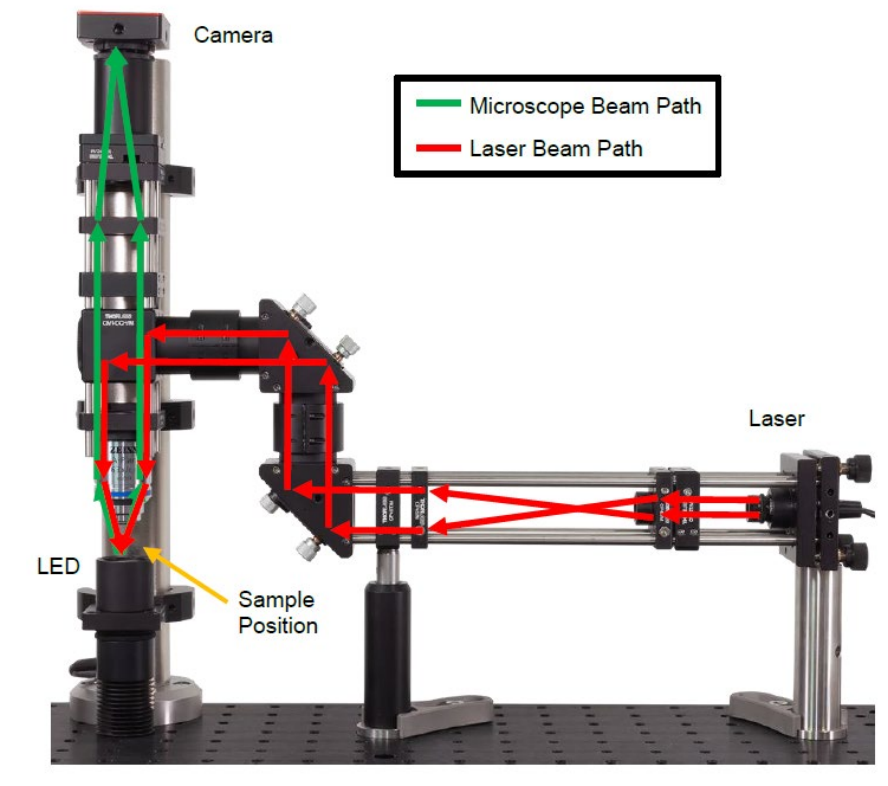
\includegraphics[angle=-90]{setup.jpg}}
        \caption{Separatory funnel}
        \label{fig:sepFunnel}
    \end{subfigure}
    \begin{subfigure}{0.49\textwidth}
        \centering
        \resizebox{0.75\textwidth}{!}{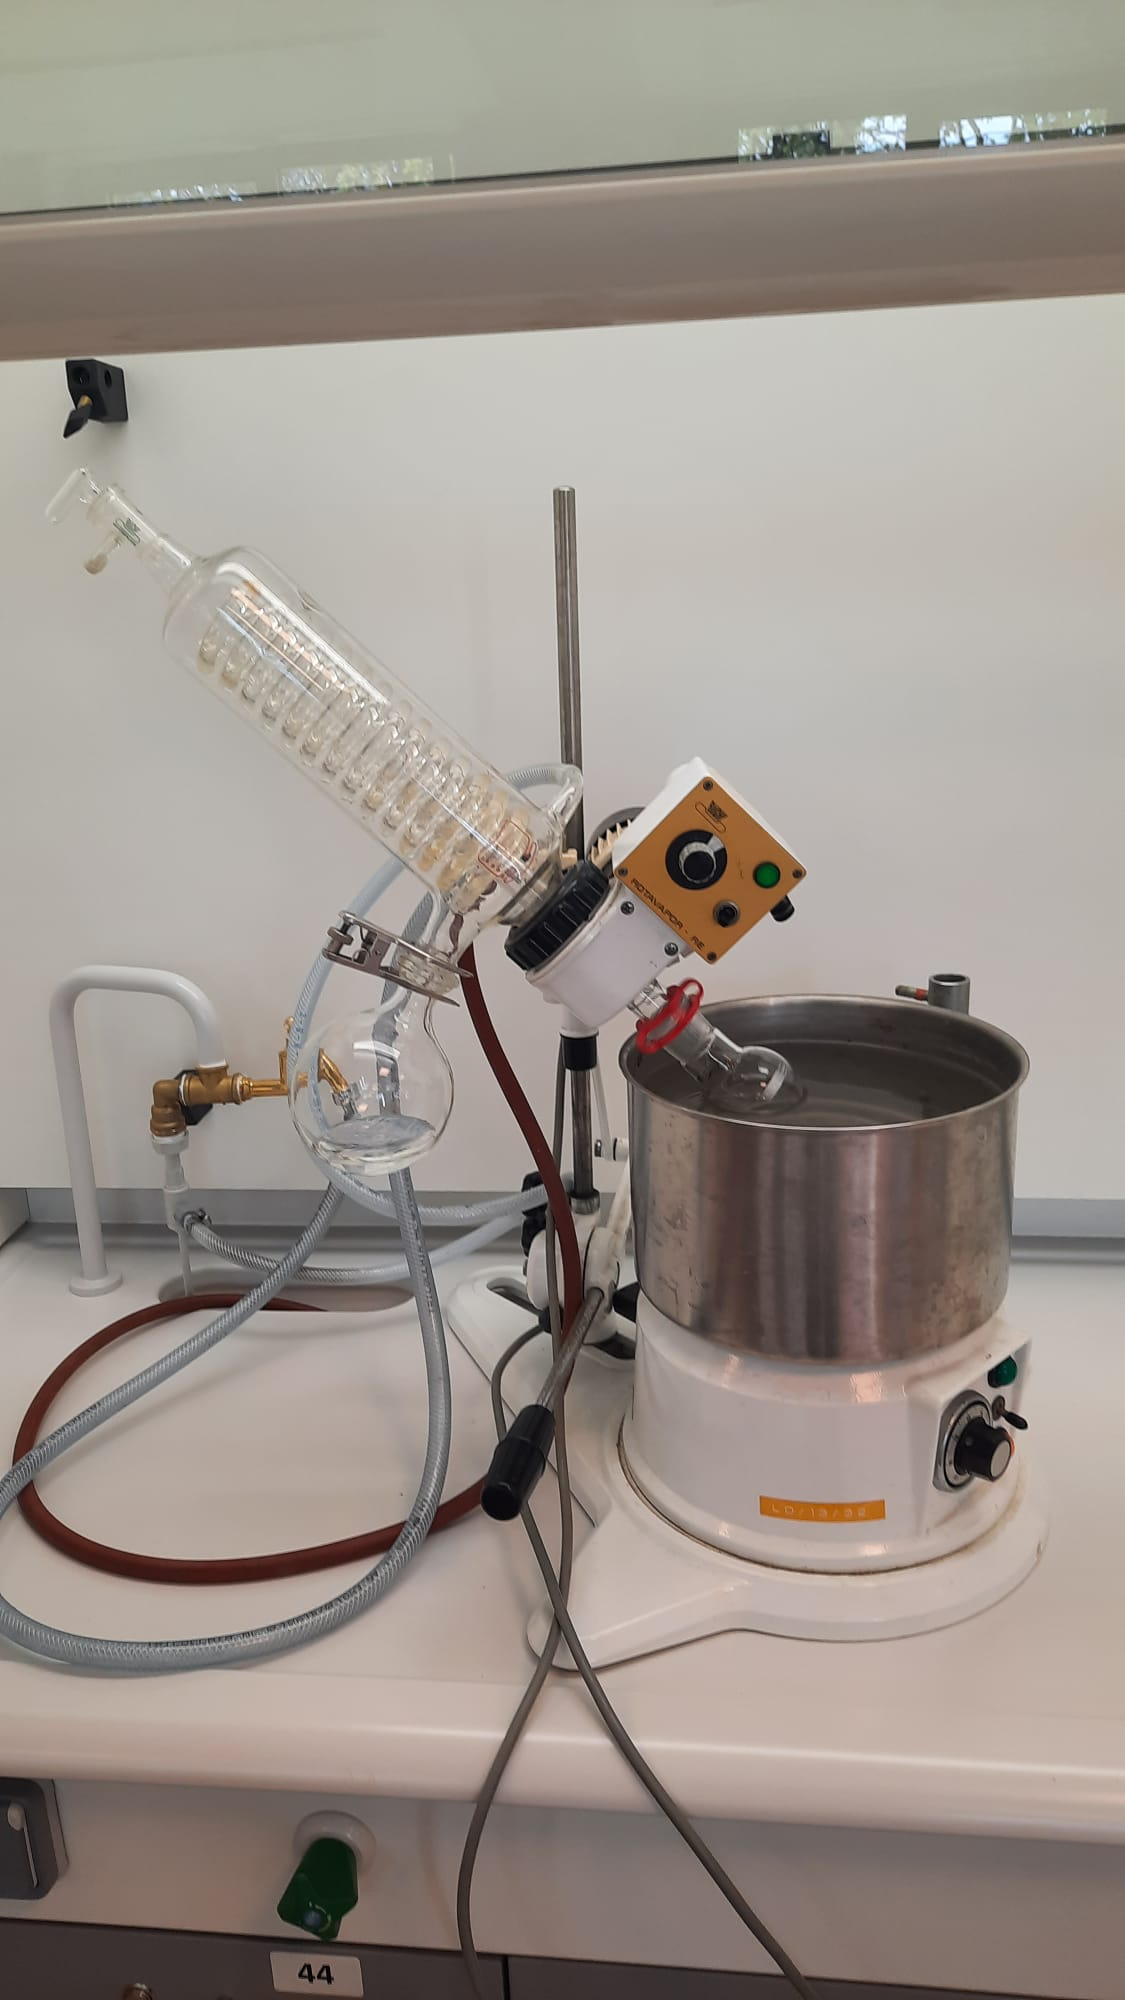
\includegraphics{rotavapor.jpg}}
        \caption{Rotavapor}
        \label{fig:rotavapor}   
    \end{subfigure}
    \caption{Experimental setups}
    \label{fig:expSetups}
\end{figure}
\FloatBarrier

\subsection{Chemicals used}

\begin{enumerate}
    \item water (\ce{H2O})
    \item potassium benzoate (\ce{C7H5KO2})
    \item benzoic acid (\ce{C7H6O2})
    \item hydrochloric acid (\ce{HCl})
    \item diethyl ether (\ce{(C2H5)2O})    
    \item sodium sulfate anhydrous (\ce{Na2SO4})
\end{enumerate}

\subsection{Safety Measures}

The standard safety equipment is in use: a lab coat, protective glasses and nitril gloves. In addition, since diethyl ether is volatile, it has to be handled under a fumehood. Also when mixing phases during the extraction, projections of solution can occur and need to be watched out for.

\section{Results and discussion}

\subsection{Liquid-liquid extraction}

\begin{wrapfigure}{l}{0.3\textwidth}
    \centering
    \resizebox{0.2\textwidth}{!}{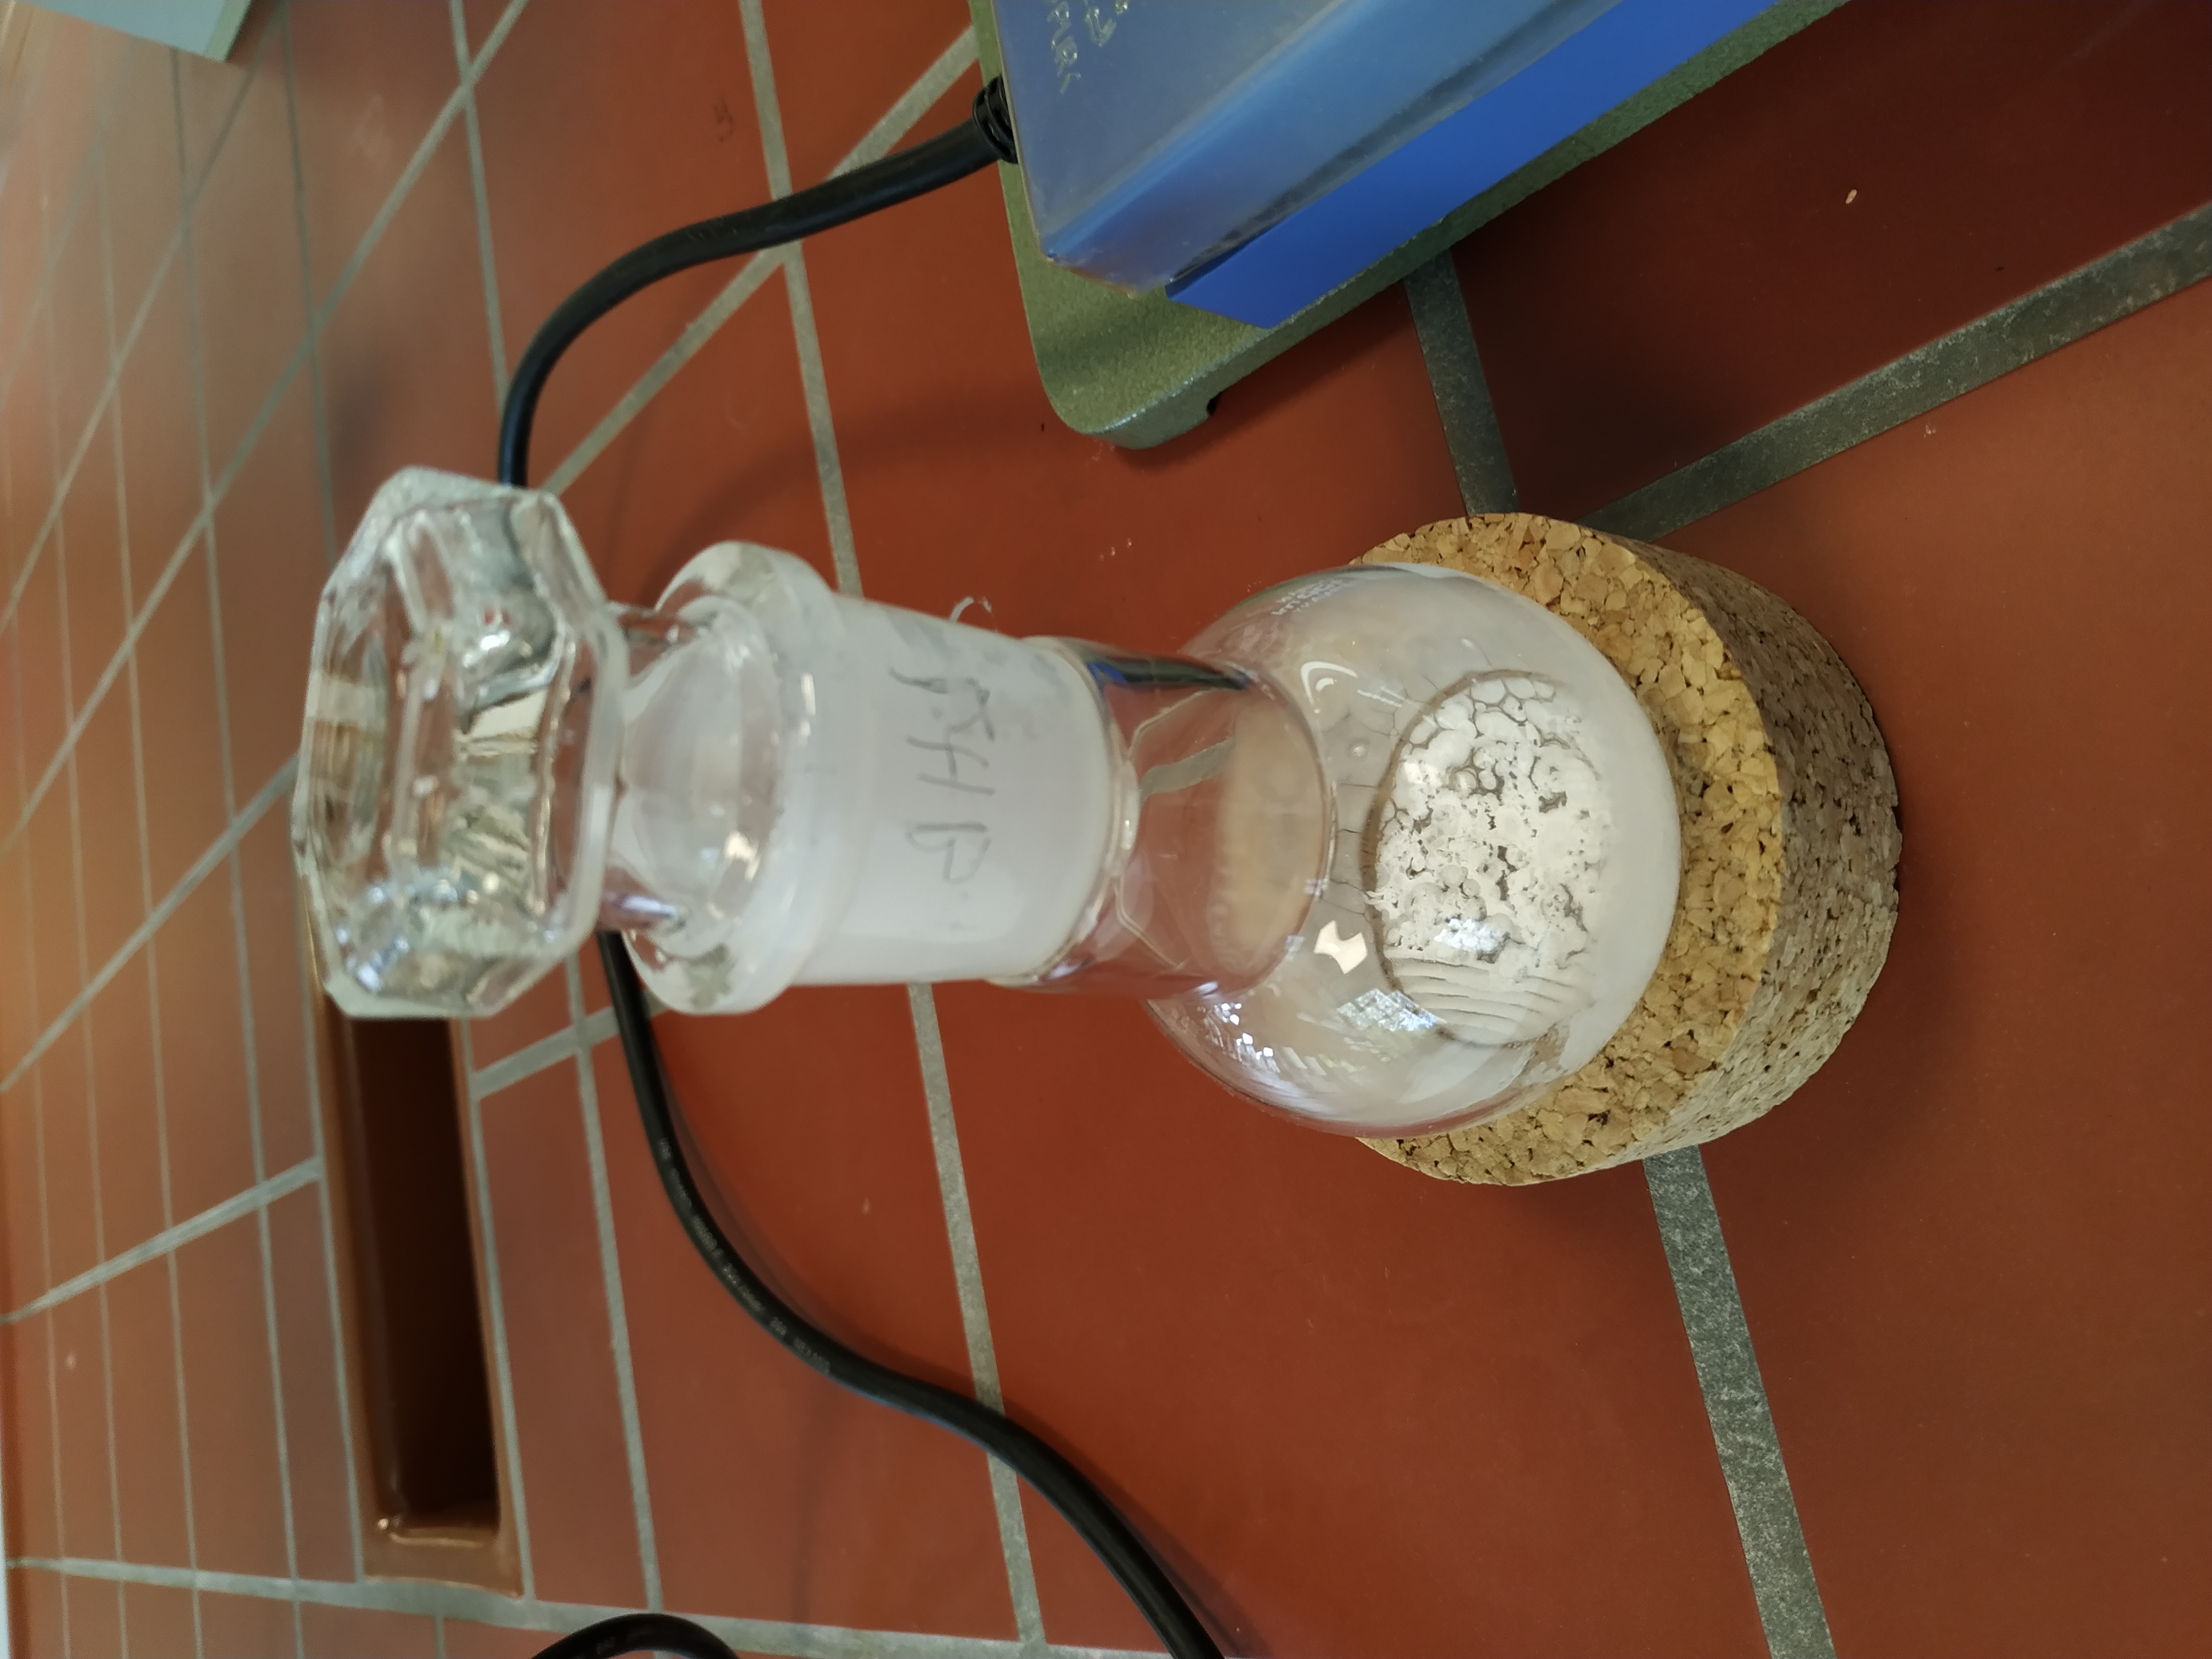
\includegraphics[angle=-90]{product.jpg}}
    \caption{Obtained benzoic acid}
    \label{fig:product}
\end{wrapfigure}

The obtained benzoic acid can be seen in  fig.\ref{fig:product}. It has formed some interesting crystal-like patterns during the evaporation: forming straight lines to the left of the flask, and blobs on the right half of the flask. This may be linked to light heterogeneity of the organic phase solution, which may have still contained water traces, or to a heterogeneous distribution of benzoic acid inside the solution. Another hypothesis is that this may be the natural way benzoic acid solidifies. 

\subsection{Yield}

The yield of the reaction is the ratio of obtained products to used reactants. In the ideal case, the yield would be close to 1, ie. as much product has been formed as reactant used. Since the stoechiometric factors are 1, the formula to calculate the yield is then given by:

\begin{equation}
    \eta = \frac{n_{\text{benzoic acid}}}{n_{\text{potassium benzoate}}}
    \label{eq:yieldFormula}
\end{equation}

Since we can only weigh the flask and the potassium benzoate, the explicit formula for the yield becomes:

\begin{equation}
    \eta = \frac{(m_{\text{flask, full}}-m_{\text{flask,empty}}) \cdot M_{\text{benzoic acid}}}{m_{\text{potassium benzoate}} \cdot M_{\text{potassium benzoate}}}
\end{equation}

The initial amount of potassium benzoate is: $m_{\text{potassium benzoate}} = 316.3$~mg. It has a molar mass of 160.213~g$\cdot$mol$^{-1}$ \cite{potassiumBenzoate}, and benzoic acid has a molar mass of 122.123~g$\cdot$mol$^{-1}$ \cite{benzoicAcid}. The empty flask weighs $76.68$~g, while after the extraction it weighs $76.91$~g The yield of the extraction is therefore:

\begin{equation*}
    \eta = \frac{(76.91~\text{g}-76.68~\text{g}) \cdot 122.123~\text{g}~\cdot~\text{mol}^{-1} }{0.32~\text{g} \cdot 160.213~\text{g}~\cdot~\text{mol}^{-1}} 
\end{equation*}

\begin{equation*}
    \boxed{ \eta = 54.78~\%}
\end{equation*}

\subsection{Melting point analysis}

The Kofler hot bench was calibrated with the substance Acetanilid. It has a melting point of 113.9°C, and the bench gave a reading of 112°C, so we have to add 2°C to find the actual melting point of the product. The measured melting point of the product is 122°C, which is about the same value as recorded in literature~\cite{MPBenzoicAcid}. The melting point analysis confirms, that the product formed is pure benzoic acid and no traces of potassium benzoate remain, as it has a melting point of  over 300°C \cite{potassiumBenzoate}, and the entirety of the sample liquefied on the bench, therefore not containing any potassium benzoate. The same argument holds for potassium chloride, which has a melting point of 770°C \cite{potassiumChloride}.

\subsection{IR spectroscopy}

A sample of the product is prelevated and studied with an IR spectrometer. The resulting spectrum can be seen in fig.~\ref{fig:IRSexp}. Its appearance is very similar to the spectrum from literature seen in fig.~\ref{fig:IRStheo}. It has the same large dip in intensity in the region of frequency corresponding to the wavenumber 3100-2300 cm$^{-1}$. The peaks present in the region of 500-2000 cm$^{-1}$ are also the same, and present the identical "double peak" structure. We can therefore conclude the product to be pure benzoic acid.

\begin{figure}[!ht]
    \centering
    \begin{subfigure}{0.45\textwidth}
        \resizebox{\textwidth}{!}{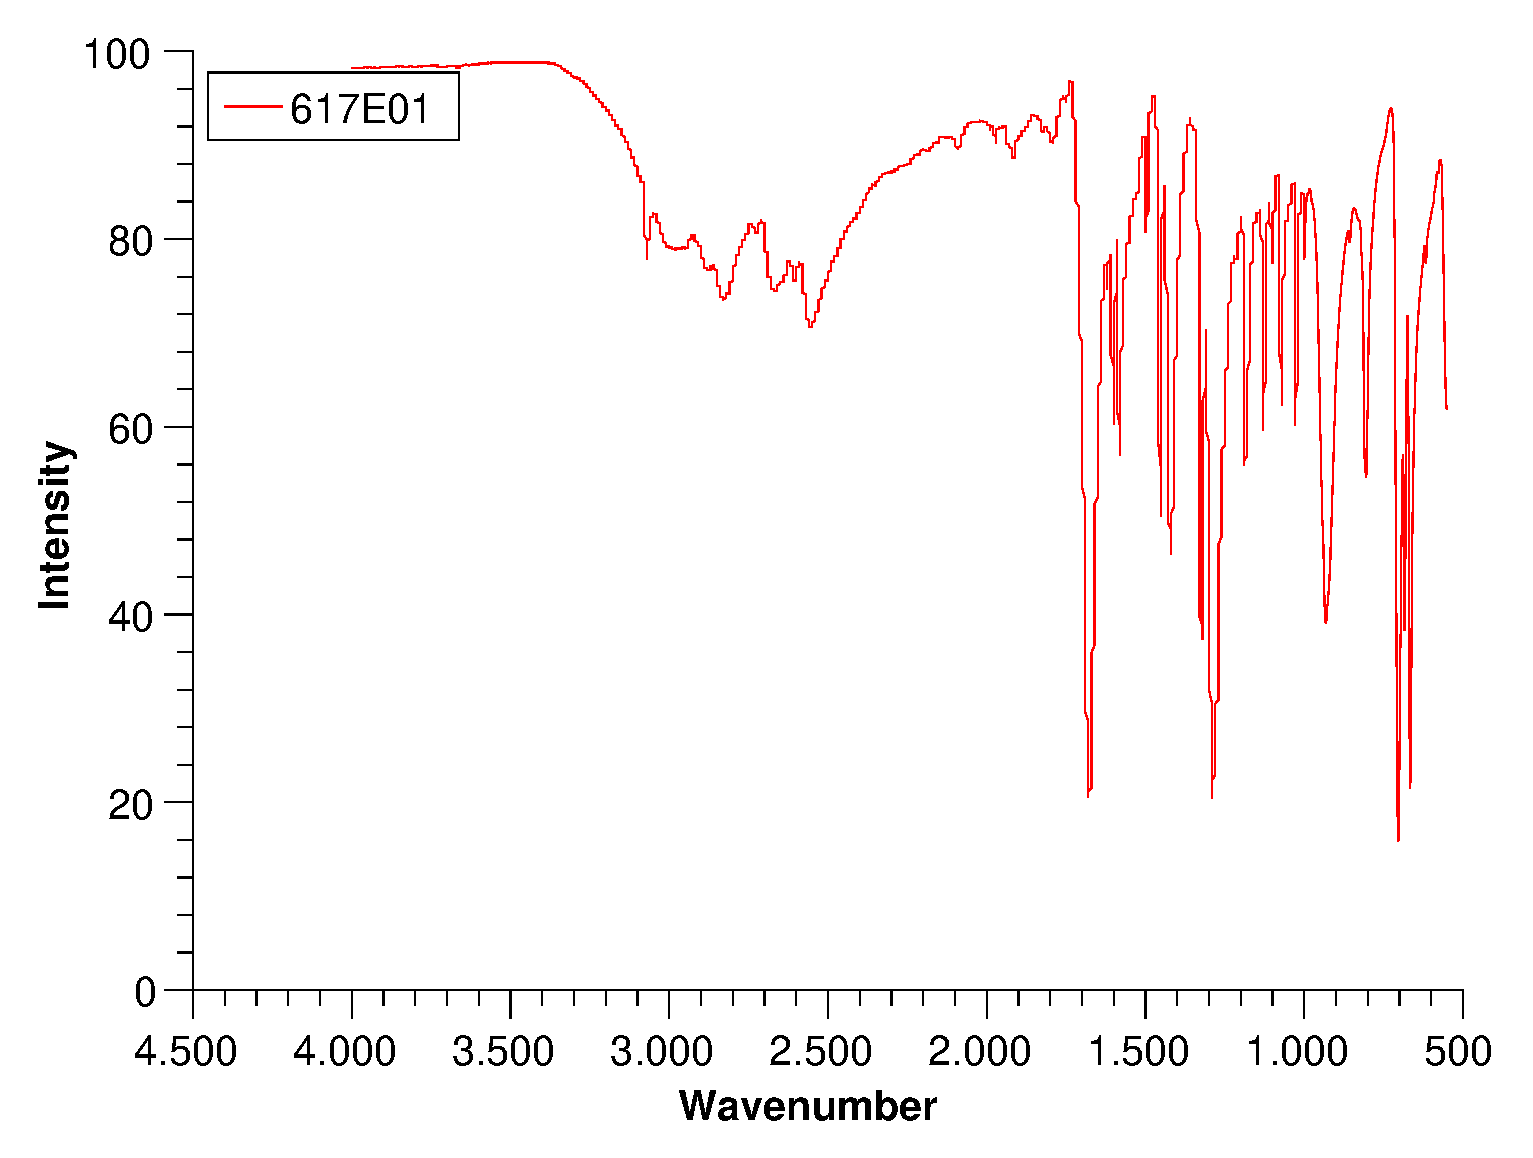
\includegraphics{IRspectrumBenzoicAcid.eps}}
        \caption{IR spectrum of the product}
        \label{fig:IRSexp}
    \end{subfigure}
    \begin{subfigure}{0.45\textwidth}
        \resizebox{\textwidth}{0.75\textwidth}{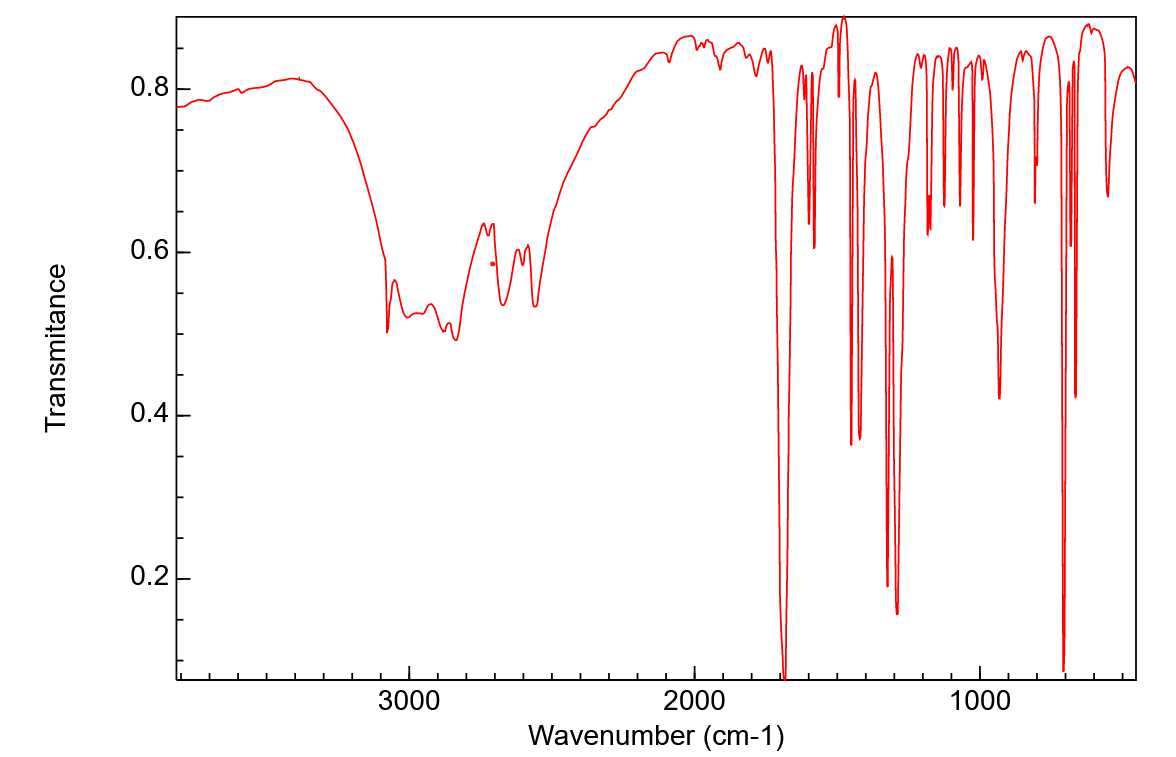
\includegraphics{IRspectrumBenzoicAcidTheo.png}}
        \caption{Theoretical IR spectrum of benzoic acid \cite{IRStheo}}
        \label{fig:IRStheo}
    \end{subfigure}
    \label{IR spectra}
    \label{IRS}
\end{figure}
\FloatBarrier

\section{Conclusion}

In this lab class we have performed the extraction of benzoic acid from potassium benzoate. This was achieved via the liquid-liquid extraction method resulting in a yield of 54.78 \%. We further identified it to be a pure product. While the yield was satisfying for the lab class, it is very inefficient for industrial standards; in order to achieve a better yield, the experiment could be improved in several ways. During the evaporation process, a very skimpy rotary evaporator was used, and we had troubles getting a good vacuum going, this probably resulted in losing some of the benzoic acid. Further sources of loss can be insufficient mixing, where doing additional extraction could have resulted in a better overall yield.

\begin{thebibliography}{}
    \bibitem{labguide} \textit{Transformation of potassium benzoate into benzoic acid}, laboratory guide, Prof. P. Dale.
    \bibitem{potassiumBenzoate} \textit{Potassium benzoate}, Wikipedia, \url{https://en.wikipedia.org/wiki/Potassium_benzoate}, last accessed 13/05/2022
    \bibitem{benzoicAcid} \textit{Benzoic acid}, Wikipedia, \url{https://en.wikipedia.org/wiki/Benzoic_acid}, last accessed 13/05/2022
    \bibitem{dichloromethane} \textit{Dichloromethane}, Wikipedia, \url{https://en.wikipedia.org/wiki/Dichloromethane}, last accessed 15/05/2022
    \bibitem{diethylEther} \textit{Diethyl ether}, Wikipedia, \url{https://en.wikipedia.org/wiki/Diethyl_ether}, last accessed 15/05/2022
    \bibitem{water} \textit{Properties of water}, Wikipedia, \url{https://en.wikipedia.org/wiki/Properties_of_water}, last accessed 15/05/2022
    \bibitem{MPBenzoicAcid} \textit{Melting point standard 121-123°C}, Sigma Aldrich \url{https://www.sigmaaldrich.com/LU/fr/product/sial/76170}, last accessed 15/05/2022
    \bibitem{IRStheo} \textit{Benzoic acid}, NIST chemistry WebBook, \url{https://webbook.nist.gov/cgi/cbook.cgi?ID=C65850&Type=IR-SPEC&Index=4}, last accessed 15/05/2022
    \bibitem{potassiumChloride} \textit{Potassium chloride}, Wikipedia, \url{https://en.wikipedia.org/wiki/Potassium_chloride}, last accessed 15/05/2022
\end{thebibliography}

\end{document}
